% metatext
The route matching algorithm is implemented by one of the \gls{astep} outdoor groups, and to check that the implementation reflects the intention a test is performed.

The implementation is tested with a sequence of routes inserted into a previous empty route database.
By adding routes sequentially, we can anticipate the matching outcome for each addition.


% test data
\textbf{Test Data}\\
A number of cases should be tested, and we generate route data for each. 
Before the route data is generated, users U1, U2, U3, and U4 are created in the \gls{astep} system.

First, the stable route generation must be confirmed functioning.
A route is created for U1 and two copies are made that were slightly edited in location and time and skewed respectively one and two weeks ahead of the original route.
These three routes should be assessed a high matching score, close to 1, and be considered a stable route for U1.

Second, the algorithm should not be matching routes that are not relevant in location or time.
U2 gets two routes added not matching in location, as seen in Figure \ref{fig:algroutes}.
The blue U2 route is during the daytime and the black during nighttime.
These routes should thus be assessed a low match score, assumed 0.

Because the algorithm should match routes of different users, we thirdly created two routes for user U3.
The routes were differencing slightly in locations and time but were made with the intention to match with each other, with one week difference in time.
The routes were also made to roughly overlap with the routes of U1, so that U1's stable route would roughly be a sub-route of the U3's route.

Lastly, the U4 route was made to discern location and time matching of the algorithm.
The route is stable and approximately at the same time as the U1 and U3 routes, but is directed in the opposite way, northwest instead of southeast.
The U4 route should match poorly with U1 and U3 routes, close to 0, but could score a bit higher, as the locations overlap with U3 route.

\begin{figure}[h]
	\centering
	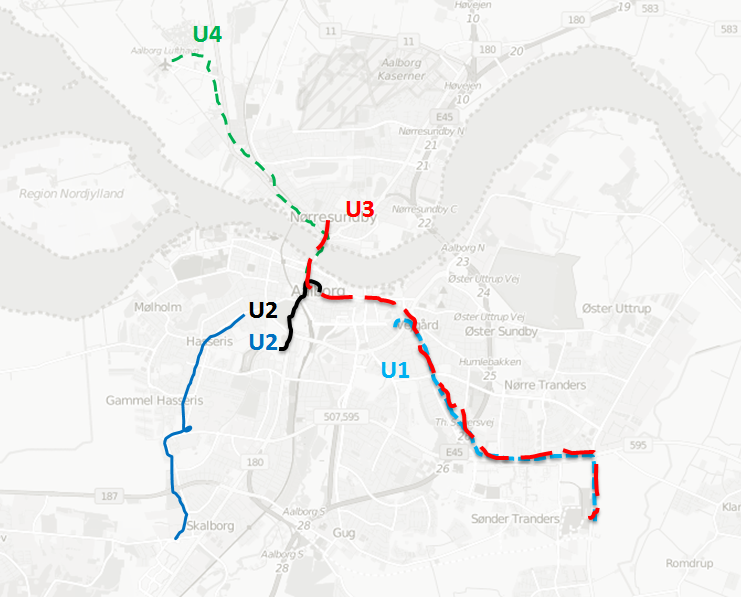
\includegraphics[width=0.7\textwidth]{figures/algorithmroutes.png}
	\caption{Generated routes to be tested by the algorithm.}
	\label{fig:algroutes}
\end{figure}


% other group executed their implemenation on test data
\textbf{Test Execution}\\
We had no influence over the actual method of the testing, but we received the following test results in Figure \ref{fig:algresults} from the outdoor group.


% test results
\textbf{Test Results}\\
The test results seen in Figure \ref{fig:algresults} reveal that the algorithm is performing correctly.
The results correspond to the assumptions made during the data generation.
All three routes of U1 are matched highly, as expected.
The U3 route is matching reasonably well with the U1 routes, and neither of the U1 routes are matching with the U3 route.
The results reflect that U3 can pick up U1 along the way while U1 will have to make a significant detour to pick up U3.

\begin{figure}[h]
	\centering
	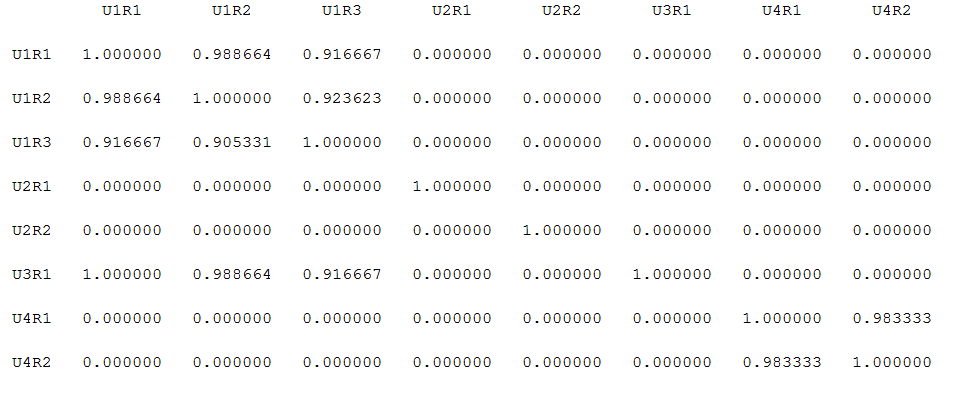
\includegraphics[width=0.8\textwidth]{figures/newtestresultrs.png}
	\caption{Results generated by the implemented algorithm.}
	\label{fig:algresults}
\end{figure}


% test results conciderations 
\textbf{Test Conclusion}\\
The algorithm test results are considered sufficient for the current application. 
However, testing, including user interviews, over large amounts of data for actual users is necessary to confirm the practical convenience of the score results.
The design of the algorithm allows adjustment of several parameter concerning distance, time and the weight of those in the final score by changing parameters in the \gls{rs} server's call to \gls{astep} system. 